\section{Исследовательский раздел} \label{research}

\subsection{Цель исследования}

Целью исследования является оценка зависимости времени выполнения запроса от наличия индексов в базе данных. Для оценки использован запрос на языке sql\cite{sql} из листинга \ref{lst:exec_time}. Необходимо определеить влияет ли использование стандартного b-tree индекса на user{\_}id  на время выполнения данного запроса при различном количестве записей.

\begin{lstlisting}[label=lst:exec_time, caption=Запрос для исследования]
select event_id, description, status, created_at, updated_at
from service.requests
where user_id={user_id};
\end{lstlisting}

\subsection{Описание исследования}

На первом этапе исследования производится замер времени выполнения запросов при количестве записей от 100 до 1000 с шагом 100 в таблице requests без использовния индекса на user{\_}id.

На втором этапе исследования производится замер времени выполнения запросов при том же количестве записей, что и на предыдущем этапе, однако с использованием индексов.

Для уменьшения погрешности вычислений каждый запрос отправляется 1000 раз, а за результат берется медианное время 1000 запросов.

Для уменьшения временных издержек, связанных с работой сети база данных и скрипт отправки запросов звпускаются на одной физической машине.

Результаты измерений приведены в таблице \ref{tab:measure}. График изображен на рисунке \ref{fig:graph}.

\pagebreak

\begin{table}[ht!]
	\centering
	\caption{Результат исследования}
	\label{tab:measure}
	\begin{tabular}{|p{4cm}|p{5cm}|p{5cm}|}
		\hline
		\textbf{Количество записей} & \textbf{Без индеков, мс} & \textbf{С индексами, мс} \\
		\hline
		100 & 9.03 & 6.91 \\
		\hline
		200 & 12.50 & 8.73 \\
		\hline
		300 & 13.41 & 10.3 \\
		\hline
		400 & 14.12 & 11.78 \\
		\hline
		500 & 15.46 & 12.13 \\
		\hline
		600 & 16.12 & 12.72 \\
		\hline
		700 & 16.42 & 12.34 \\
		\hline
		800 & 16.91 & 13.4 \\
		\hline
		900 & 17.07 & 14.23 \\
		\hline
		1000 & 17.39 & 14.10 \\
		\hline
	\end{tabular}
\end{table}

\begin{figure}[h!]
	\centering{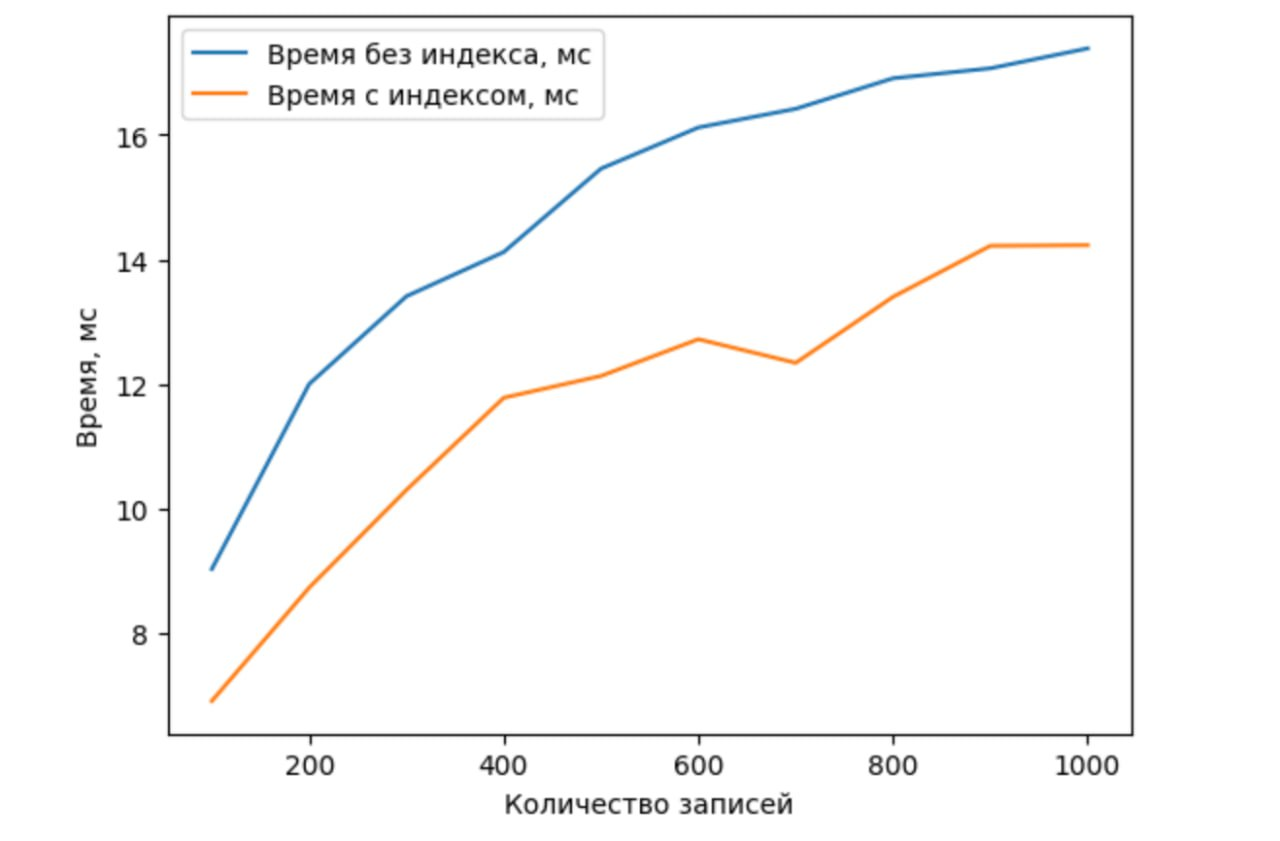
\includegraphics[scale=0.3]{img/graph.jpg}}
	\caption{График измерений}
	\label{fig:graph}
\end{figure}

\subsection{Вывод}

В результате исследования установлено, что для запроса из листинга \ref{lst:exec_time} время выполнения уменьшается при использовании индексов.

\pagebreak